\documentclass[twoside,a4paper,12pt]{uathesis}
\usepackage[percent]{overpic}
\usepackage{algorithm}
\usepackage{algorithmic}

\renewcommand{\algorithmicrequire}{\textbf{Input:}}
\renewcommand{\algorithmicensure}{\textbf{Output:}}

%make fonts searchable
%\usepackage{cmap}
%\input{glyphtounicode}
%\pdfgentounicode=1


%\usepackage[dvipsnames,table]{xcolor}
\usepackage{pgf}
\usepackage{pgfplots,pgfplotstable}
\usepackage{tikz}
\usepackage{tikzscale}
\usetikzlibrary{shapes,backgrounds}
\usetikzlibrary{arrows,shapes,fit,automata,positioning,decorations,calc}
\usetikzlibrary{spy,backgrounds}
\usetikzlibrary{arrows.meta}
\usepackage{siunitx}
\pgfplotsset{compat=1.12}


\usepackage{bbold}
\usepackage{pslatex} % -- times instead of computer modern, especially for the plain article class
%\usepackage[colorlinks=false,bookmarks=false]{hyperref}
\usepackage{booktabs}

\usepackage{multirow}
%\usepackage{cite}
\usepackage[normalem]{ulem} %for striking out text
%

\usepackage{amssymb}
\usepackage{calligra} %
\usepackage{mathtools}


\usepackage{dblfloatfix} %allows floats to be at bottom of page

%tikz and associated stuff
\usepackage{verbatim}
\usetikzlibrary{shapes,backgrounds}
\usetikzlibrary{arrows,fit,automata,positioning,decorations,calc}
\usetikzlibrary{spy}
\usetikzlibrary{matrix,chains,decorations.pathreplacing}
%\usetikzlibrary{arrows.meta}

\usepackage{caption}
\usepackage{subcaption}

\usetikzlibrary{patterns}

\usepackage[english]{babel}
\usepackage{blindtext}

\usepackage{acronym}

%\usepackage[subtle]{savetrees}

%\usepackage{flushend} % even out the last page, but use only at the end when there is a bibliography

\newcommand\defeq{\stackrel{\mathclap{\scriptsize\mbox{def}}}{=}}
\newcommand{\code}[1]{{\small{\texttt{#1}}}}

% fatter TT font
\renewcommand*\ttdefault{txtt}
% another TT, suggested by Alex
% \usepackage{inconsolata}
% \usepackage[T1]{fontenc} % needed as well?

\usepackage{listings}
\usepackage{float}
\definecolor{mygreen}{rgb}{0,0.6,0}
\definecolor{mygray}{rgb}{0.5,0.5,0.5}
\definecolor{mymauve}{rgb}{0.58,0,0.82}

\lstset{ 
  backgroundcolor=\color{white},   % choose the background color; you must add \usepackage{color} or \usepackage{xcolor}; should come as last argument
  basicstyle=\footnotesize,        % the size of the fonts that are used for the code
  breakatwhitespace=false,         % sets if automatic breaks should only happen at whitespace
  breaklines=true,                 % sets automatic line breaking
  captionpos=b,                    % sets the caption-position to bottom
  commentstyle=\color{mygreen},    % comment style
  deletekeywords={...},            % if you want to delete keywords from the given language
  escapeinside={\%*}{*)},          % if you want to add LaTeX within your code
  extendedchars=true,              % lets you use non-ASCII characters; for 8-bits encodings only, does not work with UTF-8
  frame=single,	                   % adds a frame around the code
  keepspaces=true,                 % keeps spaces in text, useful for keeping indentation of code (possibly needs columns=flexible)
  keywordstyle=\color{blue},       % keyword style
%  language=Esterel,                 % the language of the code
  morekeywords={*,...},            % if you want to add more keywords to the set
  numbers=left,                    % where to put the line-numbers; possible values are (none, left, right)
  numbersep=5pt,                   % how far the line-numbers are from the code
  numberstyle=\tiny\color{mygray}, % the style that is used for the line-numbers
  rulecolor=\color{black},         % if not set, the frame-color may be changed on line-breaks within not-black text (e.g. comments (green here))
  showspaces=false,                % show spaces everywhere adding particular underscores; it overrides 'showstringspaces'
  showstringspaces=false,          % underline spaces within strings only
  showtabs=false,                  % show tabs within strings adding particular underscores
  stepnumber=1,                    % the step between two line-numbers. If it's 1, each line will be numbered
  stringstyle=\color{mymauve},     % string literal style
  tabsize=2,	                   % sets default tabsize to 2 spaces
  title=\lstname                   % show the filename of files included with \lstinputlisting; also try caption instead of title
}
\newcommand{\todo}[1]{{\color{orange}(TODO: #1)}}
\newcommand{\hammond}[1]{{\color{blue} Hammond: #1}}
\newcommand{\matthew}[1]{{\color{red} Matthew: #1}}
\newcommand{\changed}[1]{{\color{red}#1}}

\theoremstyle{definition}
\newtheorem{definition}{Definition}[section] % definition numbers are dependent on theorem numbers
\theoremstyle{example}
\newtheorem{example}[definition]{Example} % same for example numbers
\theoremstyle{theorem}
\newtheorem{theorem}[definition]{Theorem}
\newtheorem{lemma}[definition]{Lemma}
%\newtheorem{defn}{definition}[section]
%\newtheorem{exmp}{example}[section]
%\newtheorem{rem}{remark}

\pgfplotsset{compat=1.11,
	/pgfplots/ybar legend/.style={
		/pgfplots/legend image code/.code={
			\draw[##1,/tikz/.cd,bar width=3pt,yshift=-0.2em,bar shift=0pt]
			plot coordinates {(0cm,0.8em)};
		},
	},
}



\usepackage[T1]{fontenc}
\usepackage{lmodern}
\usepackage{amsmath}
%\usepackage{amsfonts}
\usepackage{amsthm}
\usepackage{graphicx}
\usepackage[export]{adjustbox}
\usepackage{url} % format email, hypertext, and path addresses
%\usepackage[figure,linesnumbered,commentsnumbered,shortend,noline]{algorithm2e}
%\usepackage{subfigure}
\usepackage{xspace}

\usepackage{fancyvrb}
%\usepackage{bera} %for bold in verbatim 
%\usepackage{amsmath}
\usepackage{bm}

\usepackage[format=plain,labelfont=up]{caption}
\usepackage{multirow}
\usepackage{xcolor}
\usepackage{colortbl}
%\usepackage[export]{adjustbox} %used to adjust trim image
\usepackage{afterpage}
\usepackage{booktabs} %for tables to use functions such as \toprule
\usepackage{comment}

\usepackage{enumitem} %used to change enum and list spaces and settings

\usepackage{listings}
\lstset{
%     language=C,
    captionpos=b,
    breaklines=true,
%     frame=single,
    basicstyle=\footnotesize,
    numbers=left,
    numberstyle=\bf\scriptsize,
    stepnumber=1,
    numbersep=5pt,
    escapeinside={(*@}{@*)}
%     emph={solution},emphstyle={\color{red}},
%     emph={[2]phOut,oxygenOut,waterOut},emphstyle={[2]\color{blue}},
%     emph={[3]sensors,operatorStop},emphstyle={[3]\color{Green}}
}
\lstdefinelanguage{Esterel}{
    morekeywords={abort, and, await, call, case, combine, constant do, each,
                  else, elsif, emit, end, every, exec, exit, false, function,
                  halt, handle, if, immediate, in, input, inputoutput, loop,
                  mod, module, not, nothing, or,output, pause, positive, pre,
                  present, procedure, relation, repeat, return, run, sensor,
                  signal, suspend, sustain, task, then, tick, timeout, times,
                  trap, true, type, upto, var, watching, weak, when, with
                 },
    sensitive=true,
    morecomment=[l]{\%},
    morestring=[b]",
}

\usepackage{hyperref}
\hypersetup{
    pdfauthor={Keyan Monadjem},
    hidelinks
}
\usepackage{bookmark}

\newbox\subfigbox
\makeatletter
\newenvironment{subfloat}
{\def\caption##1{\gdef\subcapsave{\relax##1}}
  \let\subcapsave\@empty
  \setbox\subfigbox\hbox
  \bgroup}
{\egroup
  \subfigure[\subcapsave]{\box\subfigbox}}
\makeatother

%\newcommand{\comment}[1]{{}}
\newcommand{\dontprintsemicolon}{\DontPrintSemicolon}


%\newtheorem{definition}{Definition}
%\newtheorem{proof}{Proof}
%\newtheorem{theorem}{Theorem}

\newenvironment{abbreviations}{%
    \if@twocolumn
      \@restonecoltrue\onecolumn
    \else
      \@restonecolfalse
    \fi
    \chapter*{List of \abbreviationsname}%
      \@mkboth{\abbreviationsname}%
              {\abbreviationsname}%
  }
  {\newpage\@mkboth{}{}}
\newcommand\abbreviationsname{Abbreviations}

\begin{document}

\title{Safe Synchronous Artificial Neural Networks}
\author{Keyan Themba Monadjem}
\department{Electrical \& Computer Engineering}
\submitdate{February 2019}
\supervisor[Dr. Partha S. Roop]

%create the title page
\maketitle

%%%%%%%%%%%%% First section %%%%%%%%%%%%%%%
\frontmatter
\bookmark[page=3]{Abstract}
\include{Abstract}

\bookmark[page=5]{Acknowledgements}
\include{Acknowledgements}

%create table of contents
\bookmark[page=7]{Contents} % Sets a PDF bookmark for the contents page
\tableofcontents

\bookmark[page=11]{List of Figures}
\listoffigures

\bookmark[page=15]{List of Tables}
\listoftables

%\cleardoublepage
%\phantomsection
%\addcontentsline{toc}{chapter}{List of Abbreviations}
%\input{abbreviations}

%%%%%%%%%%%% Body of the Thesis %%%%%%%%%%%
\mainmatter

\acrodef{WCRT}{Worst Case Reaction Time}
\acrodef{WCET}{Worst Case Execution Time}
\acrodef{SOT}{Start Of Tick}
\acrodef{EOT}{End Of Tick}
\acrodef{CPS}{Cyber-Physical System}
\acrodef{AI}{Artificial Intelligence}

\acrodef{ESS}{Energy Storage System}
\acrodef{SoC}{State of Charge}
\acrodef{MBD}{Model-Based Design}
\acrodef{FPGA}{Field-Programmable Gate Array}

\acrodef{CFG}{Control Flow Graph}
\acrodef{TCFG}{Timed Control Flow Graph}
\acrodef{TCCFG}{Timed Concurrent Control Flow Graph}
\acrodef{TCA}{Tick Cost Automata}

\acrodef{SMT}{Satisfiability Modulo Theories}

\acrodef{NN}{Neural Network}
\acrodef{DNN}{Deep Neural Network}
\acrodef{SNN}{Synchronous Neural Network}
\acrodef{CNN}{Convolutional Neural Network}
\acrodef{SANN}{Synchronous Artificial Neural Network}
\acrodef{SNN}{Synchronous Neural Network}
\acrodef{SSNN}{Safe Synchronous Neural Network}
\acrodef{ANN}{Artificial Neural Network}
\acrodef{RNN}{Recurrent Neural Network}
\acrodef{MLP}{Multi-layer Perceptron}
\acrodef{MNN}{Meta Neural Network}
\acrodef{MNN2C}{Meta Neural Network to C}

\acrodef{AV}{Autonomous Vehicle}
\acrodef{LiDAR}{Light Detection and Ranging}

\acrodef{VOC}{Visual Object Classes}
\acrodef{GTSRB}{German Traffic Sign Recognition Benchmark}

\acrodef{VDTA}{Valued Discrete Timed Automata}
\acrodef{DTA}{Discrete Timed Automata}
\acrodef{RE}{Runtime Enforcement}
\acrodef{RA}{Runtime Assurance}
\acrodef{RV}{Runtime Verification}

%\include{Introduction/Introduction}
\chapter{Timing Analysis of Synchronous Neural Networks}

%\include{LiteratureReview/LiteratureReview}

%\include{Background/Backgound}

%\include{Semantics/Semantics}
%
%\include{PRET/PRET}
%

%
%\{Compilation/Compilation}
%
%\include{TimingAnalysis/TimingAnalysis}

%\include{Results/Results}

\chapter{Run-time Enforcement of Synchronous Neural Networks}

\chapter{Run-time Verification of Synchronous Neural Networks}

\section{Methodology} 
The system designed for this case study was made to reflect a \acf{AV} and its object detection mechanisms. 
The system used multiple techniques to tackle the inherent issues of the \ac{AV} system, i.e. weakness to perturbed inputs and misclassification detection.
The system's sensors include an overhead, 360$^\circ$ \acf{LiDAR} apparatus, and a single, frontal facing camera.
A solitary camera was sufficient to prove the efficacy of this solution, however it is to be noted that \ac{AV} systems generally use multiple cameras, facing different directions, so that the controller can make properly informed decisions.
The system used can be seen in Figure~\ref{fig:ssnn}. 

The \ac{LiDAR} for this system was accurate 93\% of the time~\cite{lidarFusion}, to closely simulate a real \ac{LiDAR} system.
The simulated camera outputs consisted of test images from both the \ac{VOC}~\cite{pascal-voc-2012} and \ac{GTSRB}~\cite{Stallkamp2012-gtsrb} datasets, in a combination of people, vehicles and various traffic signs.
The \ac{LiDAR} and camera outputs were handled by different parts of the controller.
The camera outputs were fed into a \ac{MNN} (see Figure~\ref{fig:mnn}) where they were classified by shape, colour and object type.

Utilising synchronous semantics, a \acf{MNN}, containing three other \ac{MNN} ensembles, was created.
Each ensemble synchronously combined the outputs of three different convolutional \acfp{SNN}~\cite{sann}, providing increased prediction accuracy for shape, colour and object type. 
These ensembles ran in synchronous concurrency, each taking four logical ticks to run. 
The outputs of each ensemble were then combined into batch of outputs forming the \textit{predicted output}. 

The system controller was encapsulated by a run-time enforcer~\cite{recps} that used sensor fusion to check for misclassifications made by the \ac{MNN}.
A safety automata (timed automata)~\ref{?} was designed to verify predictions made by the \ac{MNN} and ensure utmost safety at all times.
The automata started in a safe state, where control of the vehicle was autonomously handled by the system controller.
If a misclassification was detected, the enforced policy entered an unstable state, still under autonomous control. 
Once enough time passed without further misclassifications, the vehicle entered the safe state again.
However, if another misclassification was detected while unstable, the enforced policy entered a violation state and forced control of the \ac{AV} to the driver.
The vehicle would not enter autonomous mode again until the system was restarted.
A diagram of the enforced policy's safety (timed) automaton is shown in Figure~\ref{fig:signrte}.
This type of run-time enforcement, where neither the inputs nor outputs of the sensors or controller are enforced, has been termed as \textit{run-time verification}.
\textit{Run-time verification} refers to the verification of system parameters during run-time, while ensuring that the system is aware of any failed guards in the enforced policy.


\begin{figure}[t]
	\centering
	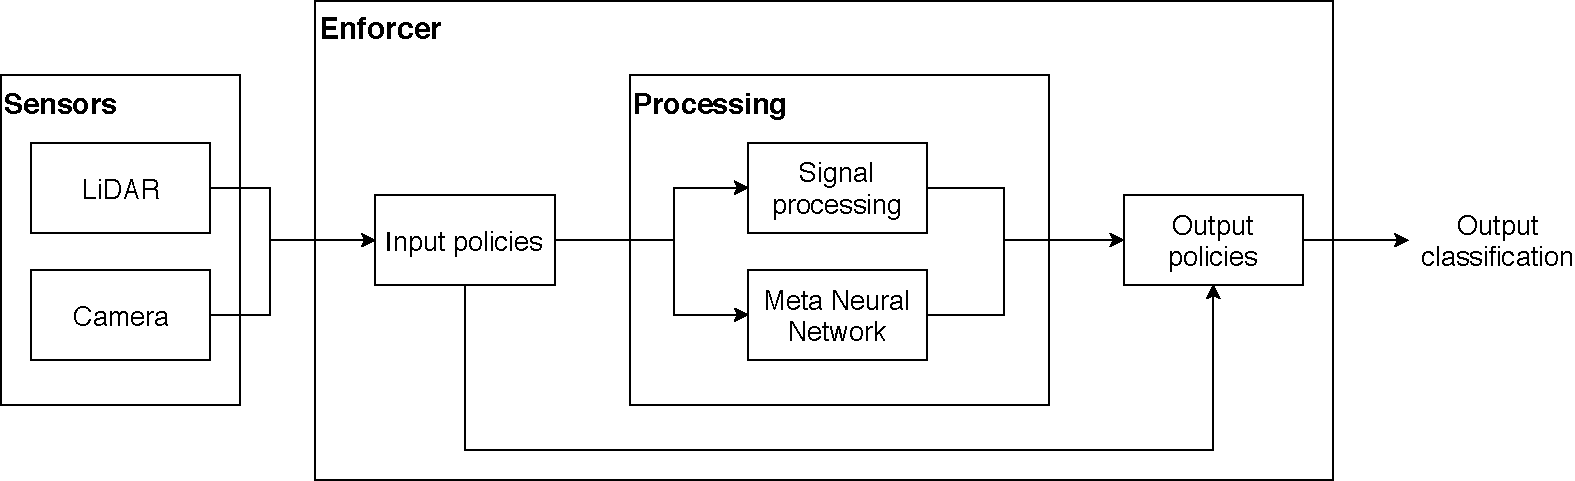
\includegraphics[scale=0.6]{Content/fig/SSNN.pdf}
	\caption{Block diagram showing the AV system with enforcer}
	\label{fig:ssnn}
\end{figure}

\begin{figure}[h]
	\centering
	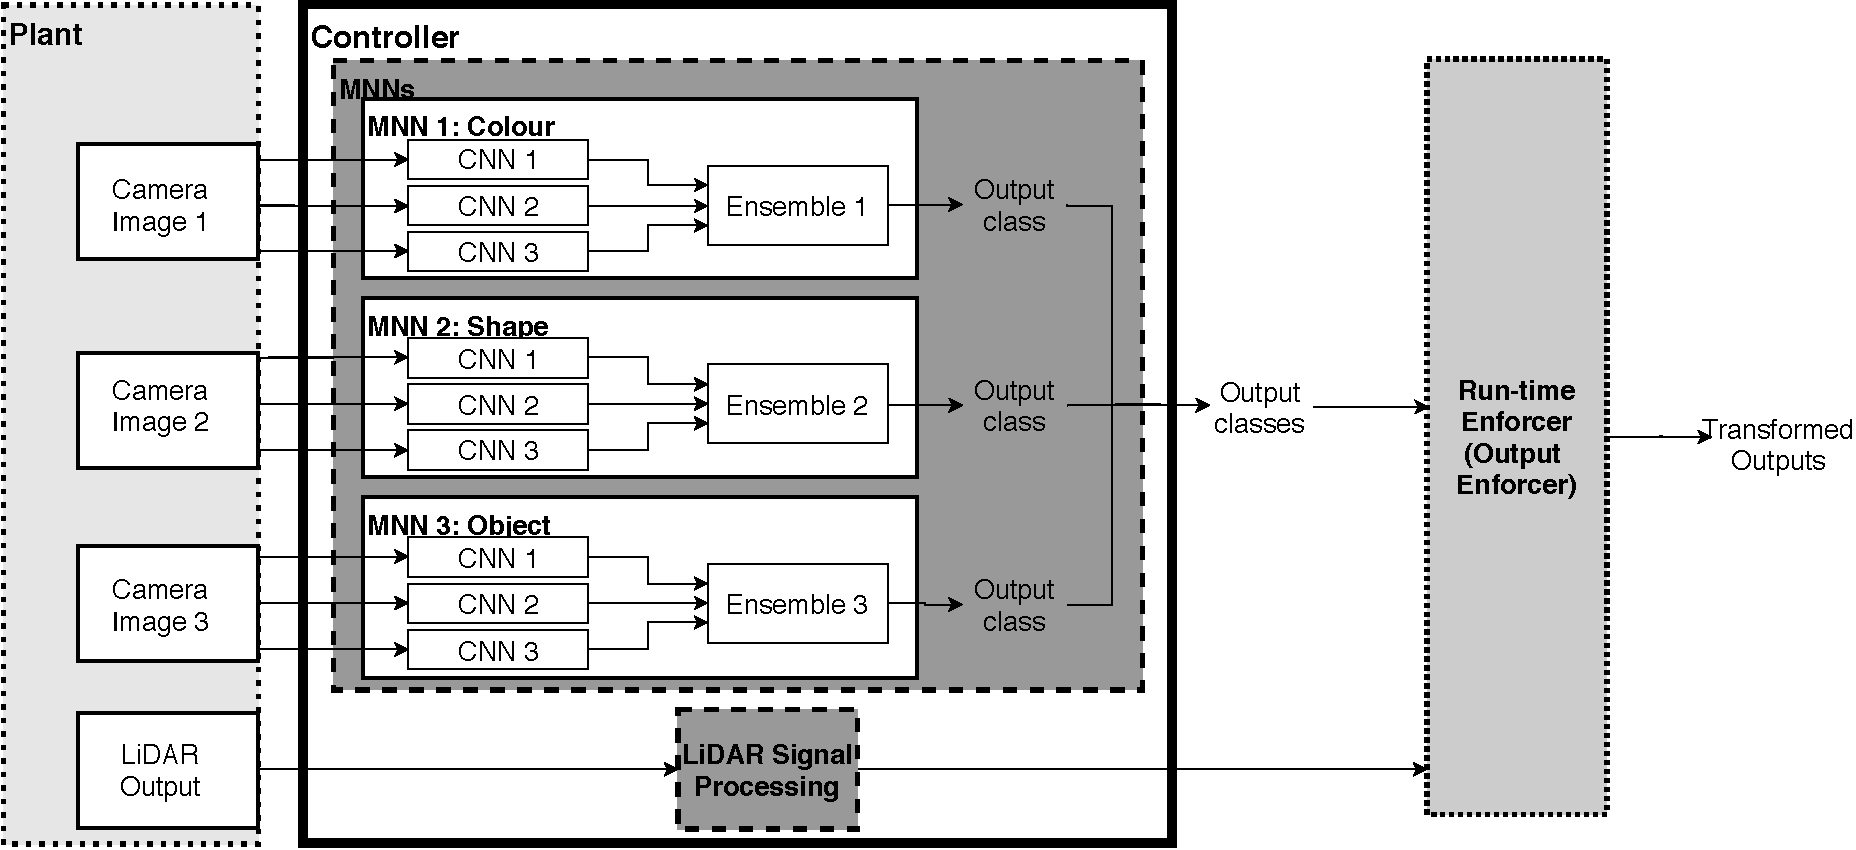
\includegraphics[scale=0.9]{Content/fig/MNN.pdf}
	\caption{Block diagram showing the Meta Neural Network ensemble} \label{fig:mnn}
\end{figure}

\begin{figure}[t]
	\centering
	\scalebox{1.3}{

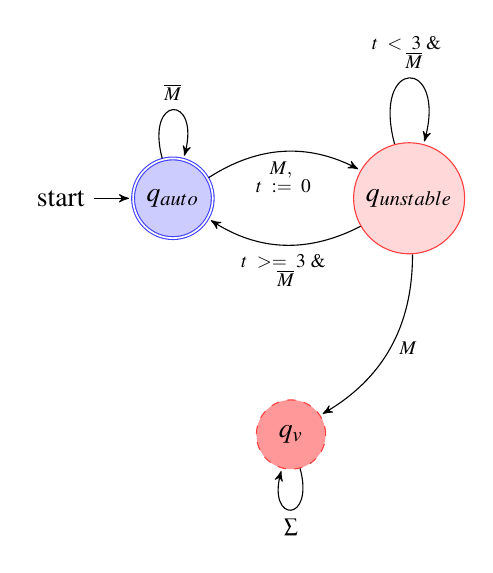
\begin{tikzpicture}[>=stealth',shorten >=1pt,auto,node distance=3 cm, scale = 1, transform shape]

\tikzstyle{accept} = [draw=blue!75,fill=blue!20]
\tikzstyle{violate} = [draw=red!75,fill=red!40, dashed]
\tikzstyle{unstable} = [draw=red!75,fill=red!15]

\node[initial,state, accepting, accept] (A) {$q_{auto}$};
\node[state, unstable] (B) [right of=A] {$q_{unstable}$};
\node[state, violate]         (C) [below of=B, xshift=-1.5cm]  {$q_v$};

\path[->] 
		(A) edge [loop above]       node [above]  
		{
			\scriptsize$\let\scriptstyle\textstyle\substack{\overline{M}}$
		} (A)
		
		(A) edge [bend left]		node [below]  
		{
			\scriptsize$\let\scriptstyle\textstyle\substack{
				M,~\\~
				t~:=~0~
			}$
		} (B)
	
		(B) edge [loop above]		node [above]  
		{
			\scriptsize$\let\scriptstyle\textstyle\substack{t~<~3~\&~\\~~\overline{M}}$
		} (B)
	
		(B) edge [bend left]		node [right]  
		{
			\scriptsize$\let\scriptstyle\textstyle\substack{M}$
		} (C)
	
		(B) edge [bend left]		node [below]  
		{
			\scriptsize$\let\scriptstyle\textstyle\substack{t~>=~3~\&\\~\overline{M}}$
		} (A)
	
		(C) edge [loop below] node [below]
		{
			\scriptsize$\sum$
		}(C)
		;

\end{tikzpicture}}

	\begin{itemize}
		\item $P$: Misclassification of a person.
		\item $V$: Misclassification of a vehicle.
		\item $N$: Classification of an object when there is nothing.
		\item $S$: Misclassification of a traffic sign.
		\item $C$: Confidence rating of the \ac{SNN} classification.
		\item $t$: Timer for the unstable state.
	\end{itemize}
	
	\caption{Enforcer policy for the AV prediction system}
	\label{fig:signrte}
\end{figure}



















\section{Results of the Runtime Verified AV System}

This research provides a solution for two aspects of \acf{AV} systems: predicting accurately with perturbations to the system's inputs and safely dealing with misclassifications by the system.
The issue of input perturbations was addressed using a \acf{MNN} of different convolutional \acfp{SNN}, each \ac{SNN} working in tandem to predict more accurately.
Misclassification by the system's controller was addressed by implementing sensor fusion between cameras and \ac{LiDAR}.
This was done using a run-time enforcer that enforced a safety automaton.

To test the \ac{MNN}'s ability to deal with perturbations, the input images (taken from the \ac{VOC} 2012 and \ac{GTSRB} datasets) were perturbed by randomly replacing approximately 7\% of the image pixels with randomly coloured pixels.
Figure~\ref{fig:sign-graph-acc} shows that the input perturbations decreased the accuracy of the classifiers by as much as 50\%, a huge amount.
However, the aim of this approach is not only to increase the classification accuracy of the \acp{SNN} but rather catch misclassifications made by the \acp{SNN}, i.e. verify that the classifications made by the \acp{MNN} are valid.
As such the results displayed don't show an increase in accuracy, but rather that the enforcer is fully capable of catching misclassifications made by the \acp{MNN}.
Table~\ref{tbl:sign-resultsfull} shows that without input perturbations, the enforcer captured more than 65\% of all misclassifications. 
This is a huge amount, more than half of all the misclassifications made were detected by the enforcer, and the safety of the system turned over to the driver.
This same table shows that when the inputs are perturbed, the enforcer picks up more misclassifications than with the original images, averaging at around 80\% of all misclassifications.
Where input perturbations are concerned, the enforcer responds even better and picks up the majority of the total misclassifications.
Figure~\ref{fig:sign-graphboth} presents these results in a graphical format, showing that the enforcer performs even better under more unpredictable circumstances.

\begin{table}[ht]
	\centering
	\caption{Table showing the results of the \ac{AV} prediction \ac{MNN}}
	\label{tbl:sign-resultsfull}
	\resizebox{\textwidth}{!}{%
		\begin{tabular}{|p{0.2\linewidth}||p{0.2\linewidth}|p{0.2\linewidth}|p{0.2\linewidth}|}
			\hline
			Epochs trained & No. of misclassifications (/100) & No. of caught misclassifications (/100) & \% of total misclassifications caught \\ \hline
			\multicolumn{4}{|l|}{Original Inputs} \\ \hline
			0 & 95.16 & 95.16 & 100 \\ 
			10 & 95.16 & 95.16 & 100 \\
			100 & 82.67 & 61.09 & 73.90 \\
			1000 & 29.36 & 21.39 & 72.85 \\
			10000 & 12.38 & 8.55 & 69.06 \\ 
			100000 & 11.98 & 7.79 & 65.03 \\
			6000 (best) & 10.59 & 7.32 & 69.12 \\ \hline
			\multicolumn{4}{|l|}{Perturbed Inputs} \\ \hline
			0 & 95.16 & 95.16 & 100 \\
			10 & 95.16 & 95.16 & 100 \\ 
			100 & 93.63 & 71.89 & 76.78 \\
			1000 & 76.69 & 63.71 & 83.07 \\
			10000 & 57.89 & 45.89 & 79.27 \\ 
			100000 & 58.03 & 45.72 & 78.79 \\
			7000 (best) & 60.42 & 49.13 & 81.31 \\ \hline
		\end{tabular}%
	}
\end{table}

\begin{figure}[t]
	\centering
	\scalebox{0.9}{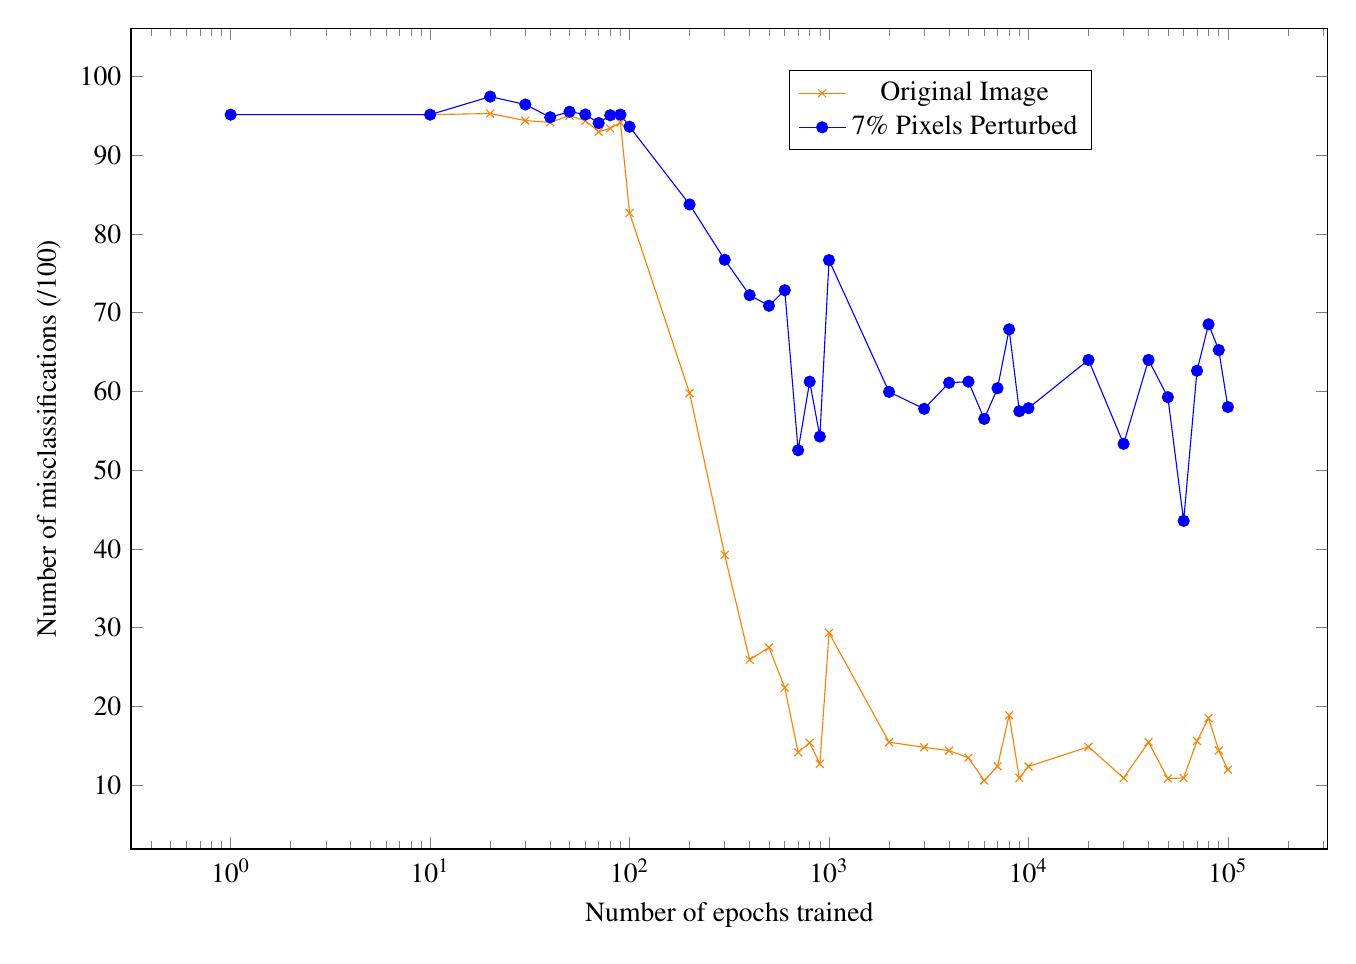
\begin{tikzpicture}
\begin{semilogxaxis}[
xlabel={Number of epochs trained},
ylabel={Number of misclassifications (/100)},
x=1.1cm,
y=1.0mm, 
legend style={at={(0.55,0.9)},anchor=west}]

\addplot[color=orange,mark=x] coordinates {
	(1, 95.159996)
	(10, 95.159996)
	(20, 95.300003)
	(30, 94.410004)
	(40, 94.180000)
	(50, 95.019997)
	(60, 94.389999)
	(70, 93.000000)
	(80, 93.419998)
	(90, 94.159996)
	(100, 82.669998)
	(200, 59.790001)
	(300, 39.240002)
	(400, 25.930000)
	(500, 27.490000)
	(600, 22.389999)
	(700, 14.180000)
	(800, 15.390000)
	(900, 12.700000)
	(1000, 29.359999)
	(2000, 15.460000)
	(3000, 14.810000)
	(4000, 14.390000)
	(5000, 13.490000)
	(6000, 10.590000)
	(7000, 12.400000)
	(8000, 18.889999)
	(9000, 10.920000)
	(10000, 12.380000)
	(20000, 14.880000)
	(30000, 10.920000)
	(40000, 15.460000)
	(50000, 10.850000)
	(60000, 10.920000)
	(70000, 15.620001)
	(80000, 18.520000)
	(90000, 14.410000)
	(100000, 11.980000)
};

\addplot[color=blue,mark=*] coordinates {
	(1, 95.159996)
	(10, 95.159996)
	(20, 97.450005)
	(30, 96.450005)
	(40, 94.830002)
	(50, 95.529999)
	(60, 95.180000)
	(70, 94.089996)
	(80, 95.089996)
	(90, 95.159996)
	(100, 93.629997)
	(200, 83.750000)
	(300, 76.729996)
	(400, 72.239998)
	(500, 70.889999)
	(600, 72.860001)
	(700, 52.540001)
	(800, 61.250000)
	(900, 54.280003)
	(1000, 76.689995)
	(2000, 59.950001)
	(3000, 57.799999)
	(4000, 61.109997)
	(5000, 61.250000)
	(6000, 56.520000)
	(7000, 60.420002)
	(8000, 67.900002)
	(9000, 57.500000)
	(10000, 57.889999)
	(20000, 64.010002)
	(30000, 53.349998)
	(40000, 64.010002)
	(50000, 59.280003)
	(60000, 43.570000)
	(70000, 62.639999)
	(80000, 68.529999)
	(90000, 65.259995)
	(100000, 58.029999)
};


\legend{Original Image, 7\% Pixels Perturbed}
\end{semilogxaxis}%
\end{tikzpicture}%}
	\caption{Line graph showing the effect of input perturbations on the prediction accuracy of a \ac{MNN} \label{fig:sign-graph-acc}}
\end{figure}

%\begin{figure}[t]
%	\centering
%	\scalebox{0.9}{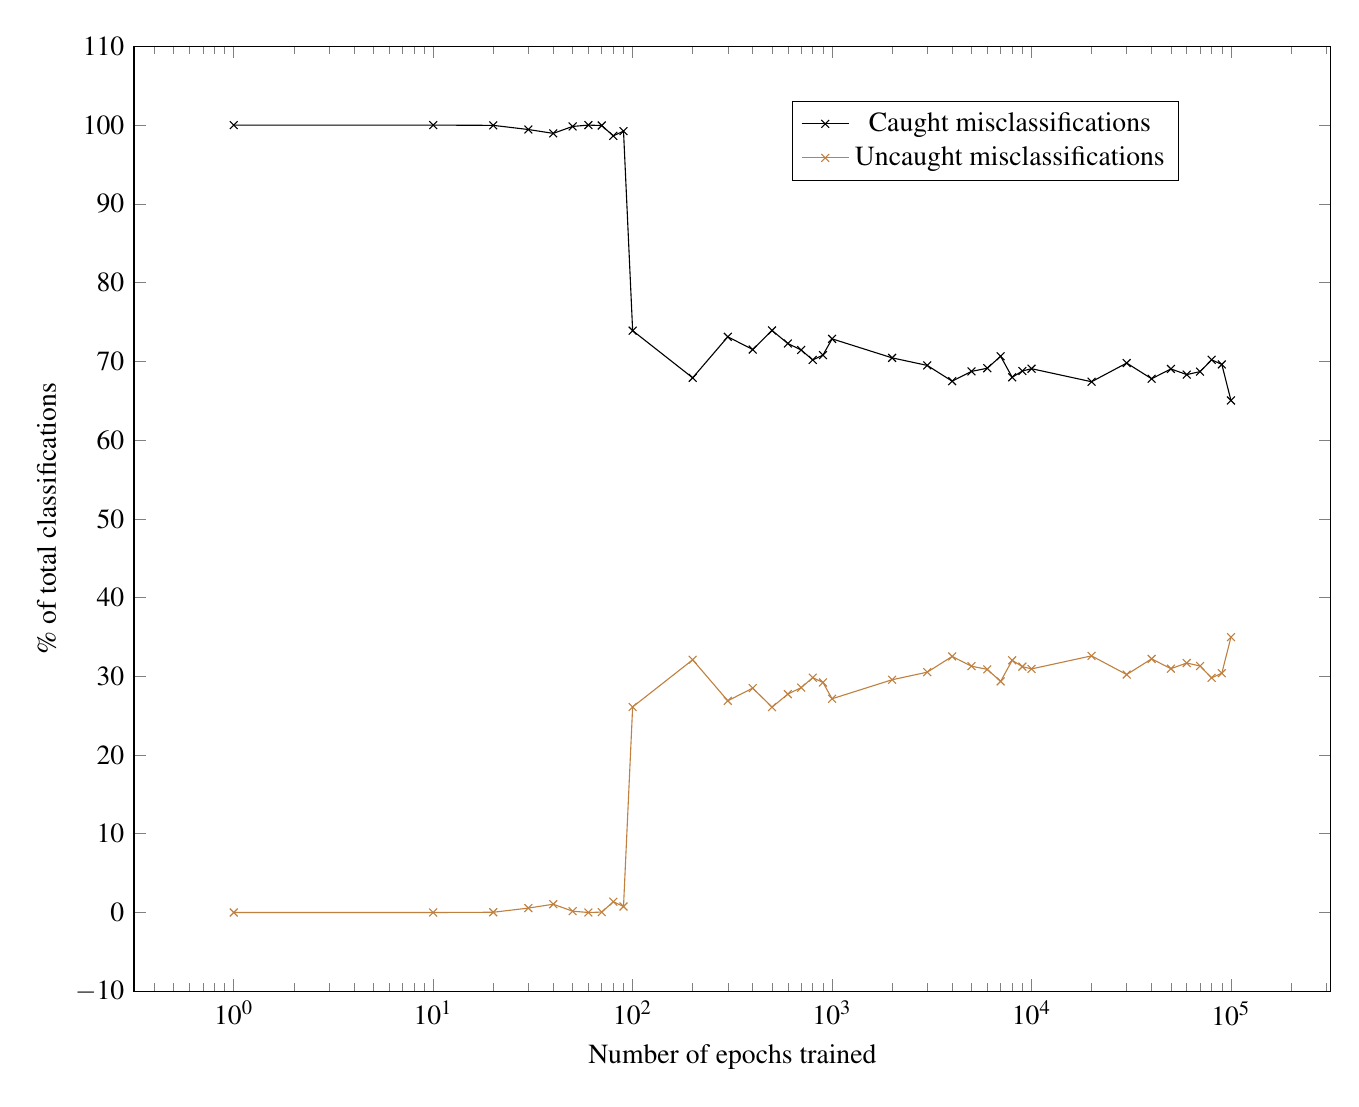
\begin{tikzpicture}
\begin{semilogxaxis}[
xlabel={Number of epochs trained},
ylabel={\% of total classifications},
x=1.1cm,
y=1.0mm, 
legend style={at={(0.55,0.9)},anchor=west}]

\addplot[color=black,mark=x] coordinates {
	(1, 100.000000)
	(10, 100.000000)
	(20, 99.968513)
	(30, 99.438622)
	(40, 98.948822)
	(50, 99.831619)
	(60, 100.000000)
	(70, 99.946243)
	(80, 98.629845)
	(90, 99.235352)
	(100, 73.896217)
	(200, 67.904327)
	(300, 73.114166)
	(400, 71.500191)
	(500, 73.917786)
	(600, 72.264412)
	(700, 71.438644)
	(800, 70.175438)
	(900, 70.787399)
	(1000, 72.854225)
	(2000, 70.439842)
	(3000, 69.480080)
	(4000, 67.477409)
	(5000, 68.717560)
	(6000, 69.121811)
	(7000, 70.645164)
	(8000, 67.972473)
	(9000, 68.772896)
	(10000, 69.063011)
	(20000, 67.405907)
	(30000, 69.780220)
	(40000, 67.787842)
	(50000, 69.032257)
	(60000, 68.315018)
	(70000, 68.693977)
	(80000, 70.194382)
	(90000, 69.604439)
	(100000, 65.025040)
};

\addplot[color=brown,mark=x] coordinates {	
	(1, 0.000000)
	(10, 0.000000)
	(20, 0.031486)
	(30, 0.561380)
	(40, 1.051184)
	(50, 0.168381)
	(60, 0.000000)
	(70, 0.053759)
	(80, 1.370155)
	(90, 0.764649)
	(100, 26.103786)
	(200, 32.095673)
	(300, 26.885832)
	(400, 28.499805)
	(500, 26.082212)
	(600, 27.735594)
	(700, 28.561354)
	(800, 29.824560)
	(900, 29.212601)
	(1000, 27.145777)
	(2000, 29.560154)
	(3000, 30.519920)
	(4000, 32.522587)
	(5000, 31.282434)
	(6000, 30.878185)
	(7000, 29.354836)
	(8000, 32.027523)
	(9000, 31.227106)
	(10000, 30.936995)
	(20000, 32.594090)
	(30000, 30.219782)
	(40000, 32.212166)
	(50000, 30.967743)
	(60000, 31.684982)
	(70000, 31.306025)
	(80000, 29.805618)
	(90000, 30.395559)
	(100000, 34.974957)
};


\legend{Caught misclassifications, Uncaught misclassifications}
\end{semilogxaxis}%
\end{tikzpicture}%}
%	\caption{Line graph showing the performance of the system trained over an increasing amount of epochs using unperturbed inputs \label{fig:sign-graph}}
%\end{figure}

%\begin{figure}[t]
%	\centering
%	\scalebox{0.9}{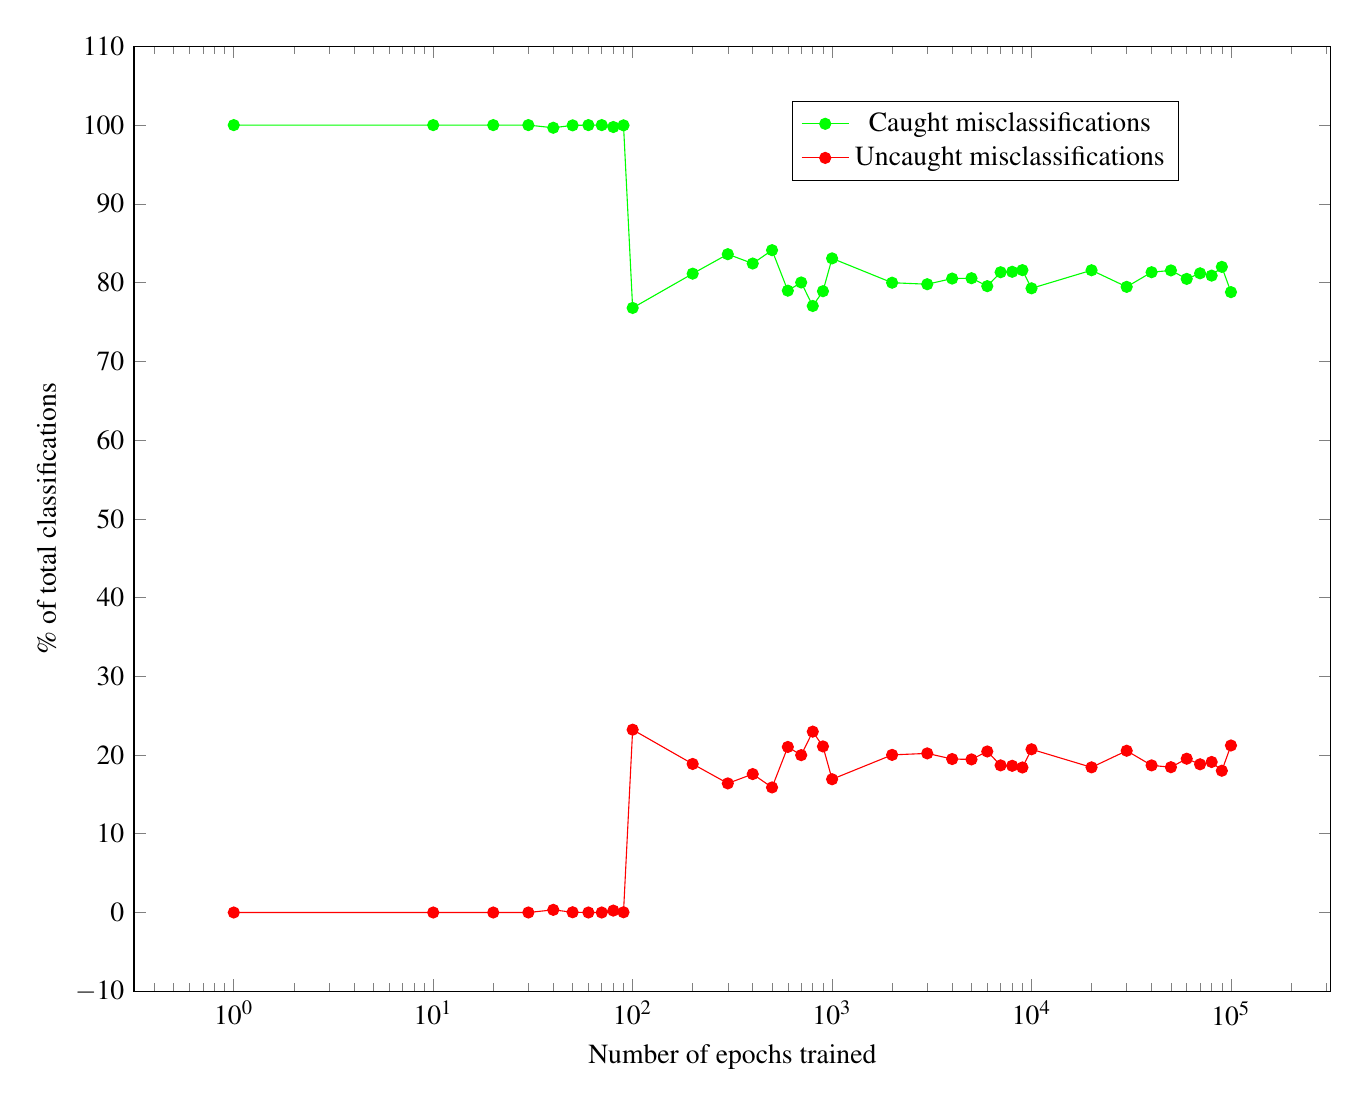
\begin{tikzpicture}
\begin{semilogxaxis}[
xlabel={Number of epochs trained},
ylabel={\% of total classifications},
x=1.1cm,
y=1.0mm, 
legend style={at={(0.55,0.9)},anchor=west}]

\addplot[color=green,mark=*] coordinates {	
	(1, 100.000000)
	(10, 100.000000)
	(20, 100.000000)
	(30, 100.000000)
	(40, 99.662552)
	(50, 99.968597)
	(60, 100.000000)
	(70, 100.000000)
	(80, 99.758133)
	(90, 99.968475)
	(100, 76.780945)
	(200, 81.134331)
	(300, 83.604851)
	(400, 82.419716)
	(500, 84.116234)
	(600, 78.973373)
	(700, 80.015221)
	(800, 77.028572)
	(900, 78.905663)
	(1000, 83.074722)
	(2000, 79.983315)
	(3000, 79.792389)
	(4000, 80.510559)
	(5000, 80.555107)
	(6000, 79.547066)
	(7000, 81.314125)
	(8000, 81.369659)
	(9000, 81.582603)
	(10000, 79.271027)
	(20000, 81.565376)
	(30000, 79.456421)
	(40000, 81.315414)
	(50000, 81.545204)
	(60000, 80.468216)
	(70000, 81.178162)
	(80000, 80.884285)
	(90000, 81.995102)
	(100000, 78.786835)
};

\addplot[color=red,mark=*] coordinates {
	(1, 0.000000)
	(10, 0.000000)
	(20, 0.000000)
	(30, 0.000000)
	(40, 0.337446)
	(50, 0.031402)
	(60, 0.000000)
	(70, 0.000000)
	(80, 0.241872)
	(90, 0.031525)
	(100, 23.219051)
	(200, 18.865665)
	(300, 16.395145)
	(400, 17.580284)
	(500, 15.883766)
	(600, 21.026627)
	(700, 19.984774)
	(800, 22.971428)
	(900, 21.094332)
	(1000, 16.925280)
	(2000, 20.016680)
	(3000, 20.207613)
	(4000, 19.489441)
	(5000, 19.444899)
	(6000, 20.452932)
	(7000, 18.685873)
	(8000, 18.630341)
	(9000, 18.417391)
	(10000, 20.728970)
	(20000, 18.434624)
	(30000, 20.543579)
	(40000, 18.684584)
	(50000, 18.454794)
	(60000, 19.531784)
	(70000, 18.821840)
	(80000, 19.115713)
	(90000, 18.004898)
	(100000, 21.213161)
};

\legend{Caught misclassifications, Uncaught misclassifications}
\end{semilogxaxis}%
\end{tikzpicture}%}
%	\caption{Line graph showing the number of misclassifications made by the system with perturbed inputs \label{fig:sign-graphpert}}
%\end{figure}

\begin{figure}[t]
	\centering
	\scalebox{0.9}{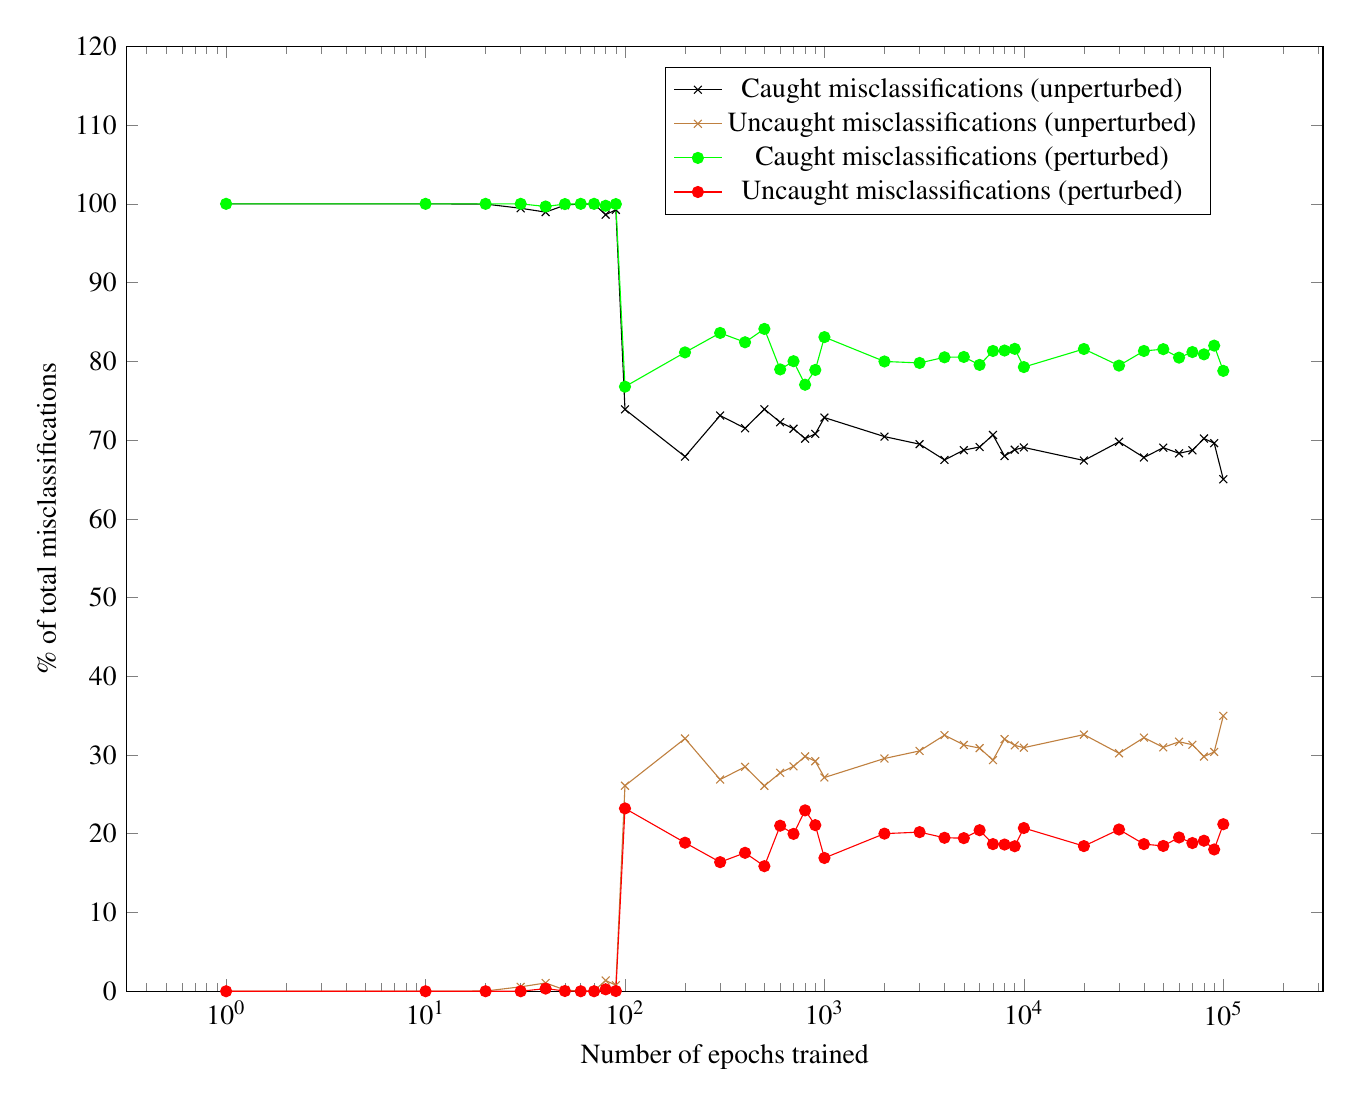
\begin{tikzpicture}
\begin{semilogxaxis}[
xlabel={Number of epochs trained},
ylabel={\% of total misclassifications},
x=1.1cm, y=1.0mm, 
ymin=0, ymax=120,
legend style={at={(0.45,0.9)},anchor=west}]

\addplot[color=black,mark=x] coordinates {
	(1, 100.000000)
	(10, 100.000000)
	(20, 99.968513)
	(30, 99.438622)
	(40, 98.948822)
	(50, 99.831619)
	(60, 100.000000)
	(70, 99.946243)
	(80, 98.629845)
	(90, 99.235352)
	(100, 73.896217)
	(200, 67.904327)
	(300, 73.114166)
	(400, 71.500191)
	(500, 73.917786)
	(600, 72.264412)
	(700, 71.438644)
	(800, 70.175438)
	(900, 70.787399)
	(1000, 72.854225)
	(2000, 70.439842)
	(3000, 69.480080)
	(4000, 67.477409)
	(5000, 68.717560)
	(6000, 69.121811)
	(7000, 70.645164)
	(8000, 67.972473)
	(9000, 68.772896)
	(10000, 69.063011)
	(20000, 67.405907)
	(30000, 69.780220)
	(40000, 67.787842)
	(50000, 69.032257)
	(60000, 68.315018)
	(70000, 68.693977)
	(80000, 70.194382)
	(90000, 69.604439)
	(100000, 65.025040)
};

\addplot[color=brown,mark=x] coordinates {	
	(1, 0.000000)
	(10, 0.000000)
	(20, 0.031486)
	(30, 0.561380)
	(40, 1.051184)
	(50, 0.168381)
	(60, 0.000000)
	(70, 0.053759)
	(80, 1.370155)
	(90, 0.764649)
	(100, 26.103786)
	(200, 32.095673)
	(300, 26.885832)
	(400, 28.499805)
	(500, 26.082212)
	(600, 27.735594)
	(700, 28.561354)
	(800, 29.824560)
	(900, 29.212601)
	(1000, 27.145777)
	(2000, 29.560154)
	(3000, 30.519920)
	(4000, 32.522587)
	(5000, 31.282434)
	(6000, 30.878185)
	(7000, 29.354836)
	(8000, 32.027523)
	(9000, 31.227106)
	(10000, 30.936995)
	(20000, 32.594090)
	(30000, 30.219782)
	(40000, 32.212166)
	(50000, 30.967743)
	(60000, 31.684982)
	(70000, 31.306025)
	(80000, 29.805618)
	(90000, 30.395559)
	(100000, 34.974957)
};

\addplot[color=green,mark=*] coordinates {	
	(1, 100.000000)
	(10, 100.000000)
	(20, 100.000000)
	(30, 100.000000)
	(40, 99.662552)
	(50, 99.968597)
	(60, 100.000000)
	(70, 100.000000)
	(80, 99.758133)
	(90, 99.968475)
	(100, 76.780945)
	(200, 81.134331)
	(300, 83.604851)
	(400, 82.419716)
	(500, 84.116234)
	(600, 78.973373)
	(700, 80.015221)
	(800, 77.028572)
	(900, 78.905663)
	(1000, 83.074722)
	(2000, 79.983315)
	(3000, 79.792389)
	(4000, 80.510559)
	(5000, 80.555107)
	(6000, 79.547066)
	(7000, 81.314125)
	(8000, 81.369659)
	(9000, 81.582603)
	(10000, 79.271027)
	(20000, 81.565376)
	(30000, 79.456421)
	(40000, 81.315414)
	(50000, 81.545204)
	(60000, 80.468216)
	(70000, 81.178162)
	(80000, 80.884285)
	(90000, 81.995102)
	(100000, 78.786835)
};

\addplot[color=red,mark=*] coordinates {
	(1, 0.000000)
	(10, 0.000000)
	(20, 0.000000)
	(30, 0.000000)
	(40, 0.337446)
	(50, 0.031402)
	(60, 0.000000)
	(70, 0.000000)
	(80, 0.241872)
	(90, 0.031525)
	(100, 23.219051)
	(200, 18.865665)
	(300, 16.395145)
	(400, 17.580284)
	(500, 15.883766)
	(600, 21.026627)
	(700, 19.984774)
	(800, 22.971428)
	(900, 21.094332)
	(1000, 16.925280)
	(2000, 20.016680)
	(3000, 20.207613)
	(4000, 19.489441)
	(5000, 19.444899)
	(6000, 20.452932)
	(7000, 18.685873)
	(8000, 18.630341)
	(9000, 18.417391)
	(10000, 20.728970)
	(20000, 18.434624)
	(30000, 20.543579)
	(40000, 18.684584)
	(50000, 18.454794)
	(60000, 19.531784)
	(70000, 18.821840)
	(80000, 19.115713)
	(90000, 18.004898)
	(100000, 21.213161)
};

\legend{Caught misclassifications (unperturbed), Uncaught misclassifications (unperturbed), Caught misclassifications (perturbed), Uncaught misclassifications (perturbed)}
\end{semilogxaxis}%
\end{tikzpicture}%}
	\caption{Line graph showing the number of misclassifications caught by the enforcer \label{fig:sign-graphboth}}
\end{figure}

\subsection{An \ac{AV} System Using \acf{MNN2C}}
\ac{MNN2C}, introduced in Section~\ref{sec:mnn2c}, creates time-predictable, modular \acfp{MNN} for C from existing Keras (with Tensorflow) trained \acp{ANN}. 
This compiler makes implementing \acfp{MNN} in C easy and safe.
For the purposes of testing and demonstration, the complex \ac{MNN} used in this chapter, shown in Figure~\ref{fig:mnn}, was trained in Python, using Keras and the exact same images used to train the original system.
This \ac{MNN} was then described in the \ac{MNN2C} format, and modular C code was generated to initialise, run and incorporate the \ac{MNN}.
To show the efficacy of \ac{MNN2C}, the generated \ac{MNN} was implemented in an identical system to the original, and run with the same tests. 
It has already been shown that \ac{MNN2C} generates outputs identical to the Keras trained \acp{ANN} with a one hundred-thousandth tolerance, so the output of each individual \ac{SNN} is not being tested, rather that the system as a whole runs as the original does.

\subsubsection{Results of an \ac{MNN2C} Generated \ac{AV} System}
Figure~\ref{fig:sign-graphboth-mnn2c} shows that the enforcer stills runs perfectly fine with Keras trained \acp{MNN} compiled to C code.
The enforcer picked up more than 70\% of all misclassifications, catching more misclassifications as the training of the \acp{MNN} was increased. 
As the training increased, the \acp{MNN} become more confident with their predictions, and thus the enforcer is able to more accurately determine misclassifications.

Since these \acp{MNN} were trained in Keras, they did not need to go through extensive training to get to a reasonable classification accuracy, only needing 100 epochs to get to level as the Darknet \acp{MNN}.
The enforcer works very similarly for perturbed and unperturbed images, unlike the Darknet \acp{MNN}.
This is due to the effective training methods used by Keras, allowing for better trained \acp{MNN} even with input perturbations.

%\begin{figure}[t]
%	\centering
%	\scalebox{0.9}{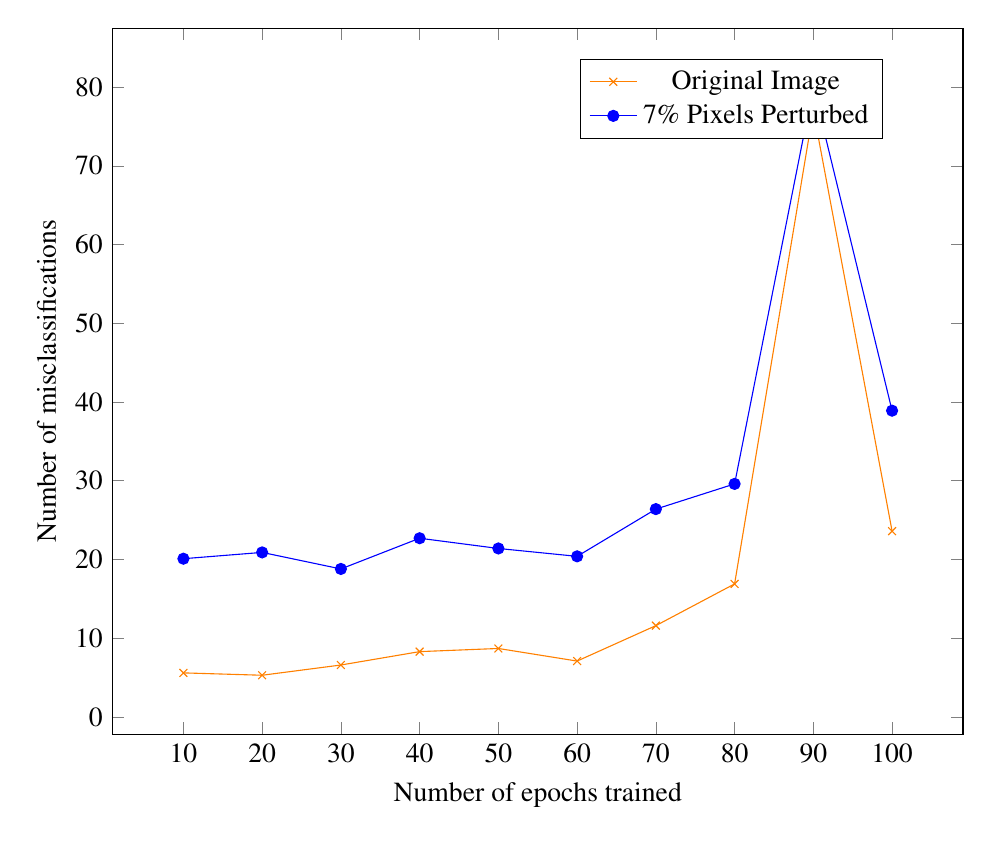
\begin{tikzpicture}
\begin{axis}[
xlabel={Number of epochs trained},
ylabel={Number of misclassifications},
x=1.0mm,
y=1.0mm, 
legend style={at={(0.55,0.9)},anchor=west}]

\addplot[color=orange,mark=x] coordinates {
	(10, 5.600000)
	(20, 5.300000)
	(30, 6.600000)
	(40, 8.300000)
	(50, 8.700000)
	(60, 7.100000)
	(70, 11.600000)
	(80, 16.900000)
	(90, 77.000000)
	(100, 23.600000)
	
};

\addplot[color=blue,mark=*] coordinates {
	(10, 20.100000)
	(20, 20.900000)
	(30, 18.799999)
	(40, 22.700001)
	(50, 21.400000)
	(60, 20.400000)
	(70, 26.400000)
	(80, 29.600000)
	(90, 80.000000)
	(100, 38.900002)
};


\legend{Original Image, 7\% Pixels Perturbed}
\end{axis}%
\end{tikzpicture}%}
%	\caption{Line graph showing the effect of input perturbations on the prediction accuracy of a \ac{SNN} \label{fig:sign-graph-acc-mnn2c}}
%\end{figure}

\begin{figure}[t]
	\centering
	\scalebox{0.9}{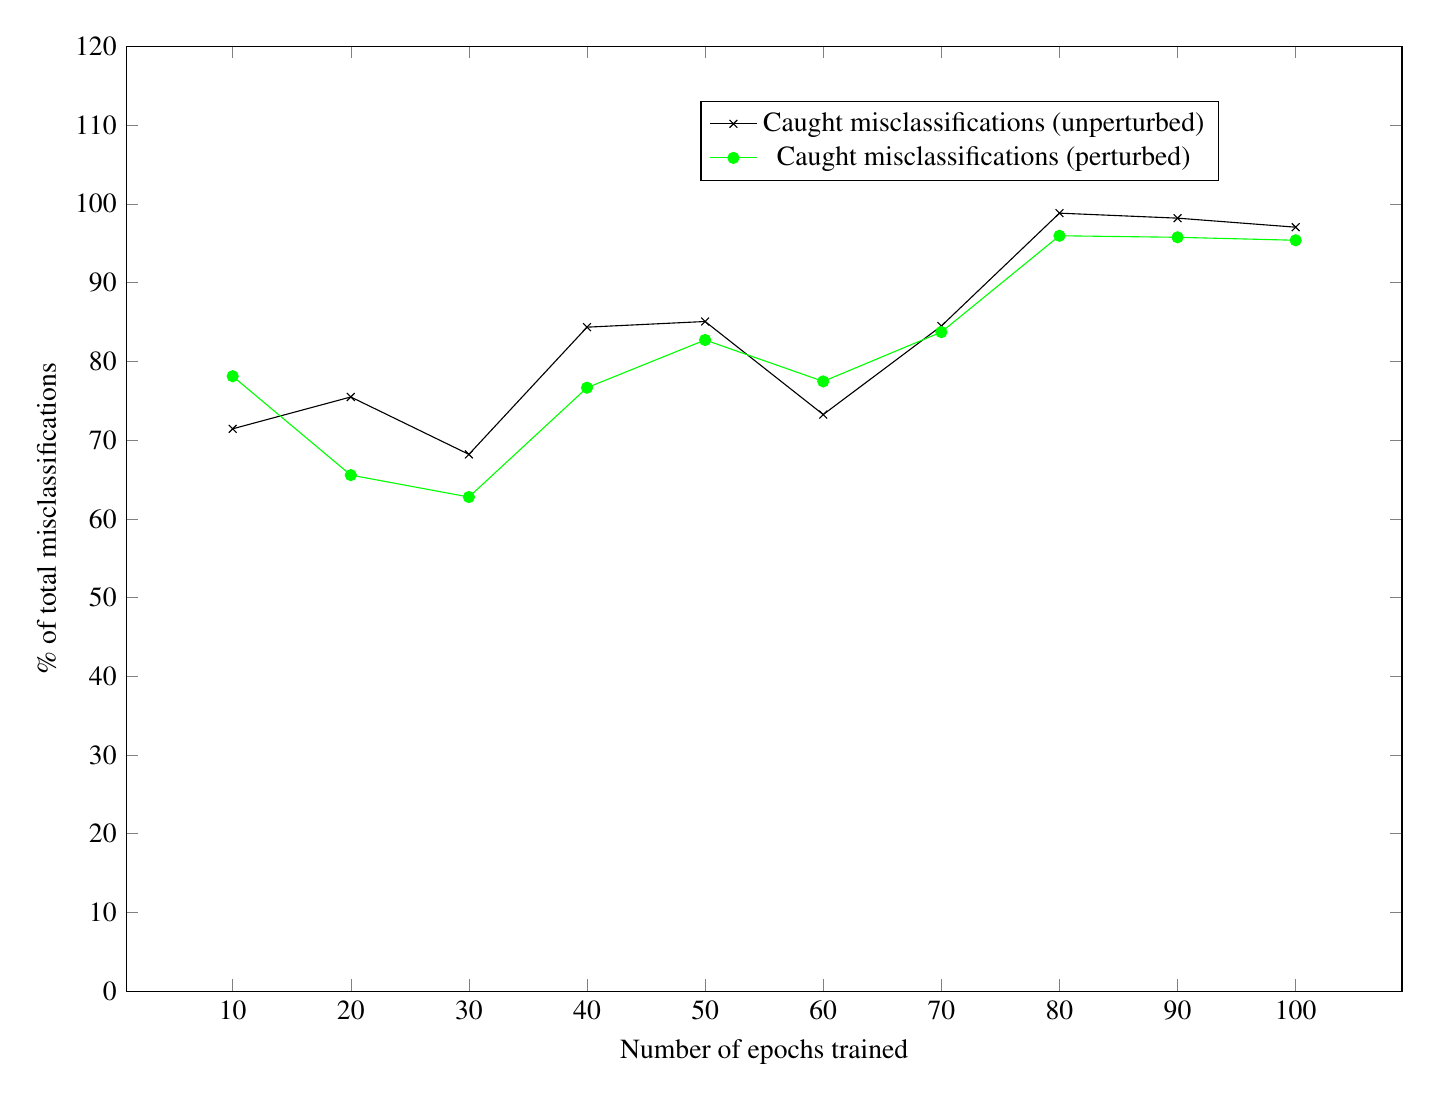
\begin{tikzpicture}
\begin{axis}[
xlabel={Number of epochs trained},
ylabel={\% of total misclassifications},
x=1.5mm, y=1.0mm, 
ymin=0, ymax=120,
legend style={at={(0.45,0.9)},anchor=west}]

\addplot[color=black,mark=x] coordinates {
	(10, 71.428574)
	(20, 75.471695)
	(30, 68.181816)
	(40, 84.337349)
	(50, 85.057472)
	(60, 73.239433)
	(70, 84.482758)
	(80, 98.816566)
	(90, 98.181816)
	(100, 97.033897)
};

\addplot[color=green,mark=*] coordinates {	
	(10, 78.109451)
	(20, 65.550240)
	(30, 62.765957)
	(40, 76.651985)
	(50, 82.710281)
	(60, 77.450981)
	(70, 83.712120)
	(80, 95.945946)
	(90, 95.750000)
	(100, 95.372749)
};

\legend{Caught misclassifications (unperturbed), Caught misclassifications (perturbed)}
\end{axis}%
\end{tikzpicture}%}
	\caption{Line graph showing the number of misclassifications caught by the enforcer with \ac{MNN2C} generated \acp{MNN} \label{fig:sign-graphboth-mnn2c}}
\end{figure}























\begin{comment}
\include{temp}
\end{comment}





%In this thesis, we proposed the use of synchronous programming towards the safe use of \acfp{ANN} in \acfp{CPS}, which are safety-critical systems.
Using the synchronous programming language Esterel, \acfp{SNN}, were developed to create \acp{ANN} that maintained synchronous semantics.
We were able to create fully synchronous, predictable \acp{ANN} that were able to be used as the controllers in all our benchmarks.
The synchronous approach to \acp{ANN}, which includes formal definitions of the \acp{ANN}, simulations and implementations of \ac{CPS}, was demonstrated throughout this thesis.
The results and concerns of this approach are discussed.

Two different structure types were defined: \acp{SNN} and \acp{MNN}.
\acp{SNN} are \acp{ANN} that run in a synchronous manner and maintain synchronous semantics, while \acp{MNN} are compositions of multiple \acp{SNN}, also retaining synchronous semantics.
Using the time predictable T-CREST platform, a set of benchmarks were developed using Esterel and C to prove the efficacy of \acp{SNN} and \acp{MNN}. 
These benchmarks ranged from basic, \acfp{MLP} to larger, more complex \acfp{MNN}.
Static timing analysis was done on these benchmarks, proving that the implemented \acp{SNN} and \acp{MNN} were not only time predictable, but also that the system were able to meet real-time deadlines.
Additionally, a Python tool chain, termed \acf{MNN2C} was introduced.
This compiler was able to produce time-predictable, \acp{MNN} from existing Keras trained \acp{ANN}.
This tool chain produced more accurate, lower \acf{WCRT} measurements compared to the original \acp{MNN}.

The next body of work introduced the concept of combining \acf{RE} with \acp{MNN}.
To this end, the definition of a \ac{MNN} was expanded to include arbitrary synchronous components, such as run-time enforcer, and not \acp{SNN}.
These new \acp{MNN} were termed \acfp{SNN}.
An \ac{AV} case study was used to demonstrate the efficacy of run-time enforced \acp{SNN} by enforcing a set of safety policies to ensure the safe behaviour of an \ac{AV} when presented with dangerous situations.
This approach was shown to vastly increase the safety of an \ac{AV}, allowing the \ac{AV} to run autonomously for long periods of time.
However, a complication arose with the realisation that the I/O of an \ac{ANN} with complex inputs, such as a \acf{CNN}, cannot be enforced.

The issue of input perturbation, where the inputs to the system are altered beyond the control of the system, was addressed next.
We proposed the use of \acf{RV}, sensor fusion and \acp{SNN} to decrease the risk posed by input perturbation.
To show the effect of input perturbation, and test our approach to addressing it, a different \ac{AV} system was created. 
This system was a simulation of the object classifier in an \ac{AV}, i.e. the part of the controller responsible for identifying the \ac{AV}'s surrounding environment.
Perturbed inputs were shown to decrease the classification accuracy of the system by up to 50\%, however our solution showed that \ac{RV} was able to ``catch'' more than 70\% of all misclassification, and when the inputs perturbation occurred the \ac{RV} was able to ``catch'' more than 80\% of the misclassifications.
Using the \ac{MNN2C} tool, this approach was tested on Keras generated \acp{SNN}.
These \acp{SNN} produced the same results, showing that more than 70\% of all misclassifications were detected by the \ac{RV}.

\section{Future Work}

While synchronous, time predictable \acp{ANN} proved to be of great value, they were only implemented and tested using C on single core processors.
The multi-core implementation and timing was not covered in thesis, but was researched with the construction of \ac{MNN2C}.
More research is required to the efficient multi-core implementations of \acp{SNN} for embedded systems.
Additionally, the hardware implementation of \acp{SNN} was not researched for this thesis, but is also a key bit of research.
\acp{SNN} have the potential to be implemented on a whole range of hardware, from \acfp{FPGA} to graphics cards.
This needs to be carefully researched. 

This thesis suggested \ac{RE} as an approach to creating safe \acp{ANN}, however only a single run-time enforcer was used in each benchmark.
While this was shown to be largely effective, this is not the limit to which \ac{RE} can be used in these \acp{SNN}.
In this thesis, we did not fully examine the enforcement of multiple networks in a \ac{SNN}, nor did we fully investigate all the possible compositions and combinations of \ac{RE} and \acp{MNN}.
Examining more compositions of \acp{SNN} with their run-time enforcers could lead to more capable systems that are still safe, or safer. 
Approaches such as using \ac{RE} during the training of \acp{SNN} has yet to be explored, and \ac{RE} between layers of individual \acp{SNN} has also yet to be explored.

Only the basics of \ac{RV} was discussed in this thesis.
\ac{RV} has a lot more value than just being used for \acp{CNN} in \ac{AV} systems.
This approach can be taken on any system where the inputs to the system are complex, such a intrusion detection system on networks. 
More benchmarks should be developed that expand on a lot more \ac{CPS} that could benefit from \ac{RV}.

Lastly, the composition of \acp{SNN} was not fully researched in this thesis.
The training phase of \acp{SNN} was skipped, instead each \ac{ANN} was trained individually.
\acp{SNN} are a unique composition of \acp{SNN} and other synchronous components, and the training of such systems needs further investigation.
Additionally, the only structure of \ac{SNN} used in this thesis was a \ac{SNN} ensemble, where each \ac{SNN} in the ensemble works with the others in the ensemble to provide more accurate output.
There exist endless ways that \acp{SNN} can be combined, and more of these ways should be implemented and tested.












\appendix
\chapter{Appendix}


%\include{Publications}


%%%%%%%%%%%% Last part of thesis indices, bibliography  %%%%%%%%%%%%
\backmatter

%create the bibliography
% \bibliographystyle{siam}
\renewcommand{\bibname}{References}
% \clearpage
\phantomsection
\addcontentsline{toc}{chapter}{\bibname}
\bibliographystyle{IEEEtranS}
\bibliography{references}


\end{document}

